\documentclass[border=.2cm]{standalone}
\usepackage{tikz}
\usepackage{amsmath}
\usetikzlibrary{angles}

\begin{document}

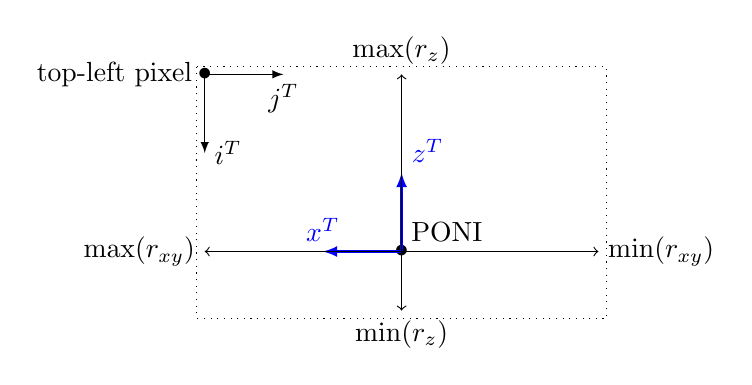
\begin{tikzpicture}[axis/.style={->,>=latex,blue,thick}]
    \draw[->,>=latex] (0,0) coordinate(O) node[anchor=east,xshift=-1] {top-left pixel} -- (1,0) node[anchor=north] {$j^T$};
    \draw[->,>=latex] (O) node[] {$\bullet$} -- (0,-1) node[anchor=west] {$i^T$};
    \draw[dotted] (-0.1,.1) -- (5.1,.1) -- (5.1,-3.1) -- (-.1,-3.1) -- cycle;
    \draw (2.5,-2.25) coordinate(O2) node {$\bullet$} node[anchor=south west] {PONI};
    \draw[axis] (O2) --++ (0,1) node[anchor=south west] {$z^T$};
    \draw[axis] (O2) --++ (-1,0) node[anchor=south] {$x^T$};
    \draw[->] (O2) --++ (-2.5,0) coordinate (y) node[left] {$\text{max}(r_{xy})$};
    \draw[->] (O2) --++ (0,2.25) coordinate(z) node[above] {$\text{max}(r_z)$};
    \draw[->] (O2) --++ (2.5,0) node[right] {$\text{min}(r_{xy})$};
    \draw[->] (O2) --++ (0,-.75) node[below] {$\text{min}(r_z)$};
\end{tikzpicture}

\end{document}

